\section{Durchführung}
\label{sec:Durchführung}

\subsection{Aufbau}

Der schematische Versuchsaufbau ist in Abbildung \ref{fig:aufbau1} dargestellt. Die einzelnen Bauteile und deren Funktion werden im Folgenden genauer beschrieben. Die 
Funktionsweise des Szintillators wurde bereits im Kontext des Abschnittes \ref{sec:Theorie} beeschrieben, weshalb hier nicht genauer darauf eingegangen wird.

\begin{figure}
    \centering
    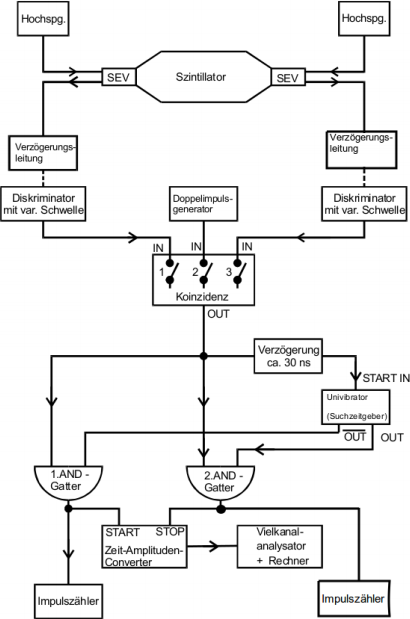
\includegraphics[width=\textwidth]{data/aufbau_skizze_1.png}
    \caption{Schematischer Aufbau des Versuchs}
    \label{fig:aufbau1}
\end{figure}

Die Signale, welche vom Szintillator an die Photomultiplier (PMT) weitergeleitet werden, sind durch Energieniveauübergänge entstehende Photonen. Diese treffen zuerst auf eine Photokathode,
wodurch ein Elektron emittiert wird, welches dann auf mehrere hintereinander geschaltete Elektroden unter Hochspannung trifft und somit Sekundärelektronen auslöst, um einen messbaren
Ladungsimpuls zu erzeugen. Es kann nicht davon ausgegangen werden, dass die beiden Photomultiplier die exakt gleiche Ansprechzeit haben, weshalb dies über eine Verzögerungsleitung 
angepasst wird. Noch vor der Verzögerungsleitung wird außerdem auf beiden Seiten jeweils ein Diskriminator eingebaut, der dafür sorgt, dass ein Untergrundrauschen unterdrückt wird.
Die auf diese Weise modifizierten Signale treffen dann von beiden Seiten auf eine Koinzidenzschaltung, die nur dann ein Signal weitergibt, wenn es von beiden Seiten gleichzeitig,
bzw. innerhalb eines Zeitintervalls $\Delta t_\text{K} $ ankommt. 
Danach folgen in der Schaltung zwei AND-Gatter, die im Zusammenspiel mit einem Monoflop dazu dienen, ein Startsignal von einem Stoppsignal unterscheiden zu können. beide AND-Gatter
sind sowohl direkt mit der Koinzidenz, als auch an den Monoflop, der wiederum über eine $\SI{30}{ns}$ Verzögerungsleitung mit der Koinzidenz verbunden ist. Die Signale der beiden 
AND-Gatter werden dann jeweils einzeln gezählt, wobei die Signale des einen die Startsignale, und die des anderen die Stoppsignale angeben. Beide AND-Gatter sind außerdem mit 
dem dahinter befindlichen Time-Amplitude-Converter (TAC) verbunden, der die Dauer zwischen einem Startsignal und einem Stoppsignal misst, um diese in eine Spannung zu 
übersetzen. Von da aus werden die Signale weiter an den Multi-Channel-Analyzer (MAC) und den zur Auswertung der Messwerte notwendigen PC gegeben. Mit diesem Aufbau kann 
gewährleistet werden, dass ein Signal eines eintreffeden Myons von dem eines Zerfalls unterschieden wird, um somit die individuellen Lebensdauern der Myonen messen zu können. 